% Template for ICASSP-2021 paper; to be used with:
%          spconf.sty  - ICASSP/ICIP LaTeX style file, and
%          IEEEbib.bst - IEEE bibliography style file.
% --------------------------------------------------------------------------
\documentclass{article}
\usepackage{spconf,amsmath,graphicx,csquotes,siunitx}
%\addbibresource{refs.bib}

% Example definitions.
% --------------------
\def\x{{\mathbf x}}
\def\L{{\cal L}}

% Title.
% ------
\title{Transfer Learning using Musical/Non-Musical Mixtures for Multi-Instrument Recognition}
%
% Single address.
% ---------------
%\name{(s)\thanks{Thanks to the Austrian Research Promotion Agency (FFG) for partially %funding.}}
%\address{Author Affiliation(s)}
%
% For example:
% ------------
%\address{School\\
%	Department\\
%	Address}
%
% Two addresses (uncomment and modify for two-address case).
% ----------------------------------------------------------
\twoauthors
  {H. Bradl, F. Pernkopf\sthanks{Thanks to the Austrian Research Promotion Agency (FFG) for partial funding.}}
	{Graz University of Technology\\
	Signal Processing and Speech Communication Lab.}
  {M. Huber}
	{sonible GmbH\\
	Graz, Austria}
%
\begin{document}
\ninept
%
\maketitle
%
\begin{abstract}
%todo: 100-150 words
Datasets for most music information retrieval (MIR) tasks tend to be relatively small. However, in deep learning, insufficient training data often leads to poor performance. Typical ways to overcome this problem are transfer learning (TL) as well as data augmentation. In this work, we compare various of these methods for the task of multi-instrument recognition. The classifier, a convolutional neural network (CNN) operating on mel-spectrogram representations of short audio chunks, is able to identify eight instrument families and seven specific instruments from polyphonic music recordings. Training is conducted in two phases: After pre-training with a music tagging dataset, the CNN is retrained using three multi-track datasets. %For this reason, we experimented with different TL methods. 
Experimenting with different TL methods suggests that training the final fully-connected layers from scratch while fine-tuning the convolutional backbone yields the best performance. Training examples are produced on-the-fly by mixing of single-instrument tracks from the multi-track datasets. Two different mixing strategies -- musical and non-musical mixing -- are investigated. It turns out that a blend of both mixing strategies works best for multi-instrument recognition. The final classifier shows state-of-the-art F1-scores for classes with sufficient training data.
\end{abstract}
%
\begin{keywords}
Multi-Instrument Recognition, Transfer Learning, Convolutional Neural Network
\end{keywords}
%
\section{Introduction}
\label{sec:intro}
Instrument recognition is an important task in MIR. The goal of early research was to identify single instruments in monophonic recordings. This task was usually approached using hand-crafted features and traditional machine learning algorithms~\cite{eronen2000musical, david2004efficient}. Later, research shifted to predominant instrument recognition in polyphonic recordings. Only recently, people started to think about the ultimate goal of instrument recognition; namely multi-instrument recognition – whose aim is to identify all instruments in a polyphonic mixture. Formally, this is a multi-label classification problem since multiple mutually non-exclusive labels can be assigned to each instance. Lately, deep learning became the preferred way to tackle multi-instrument recognition and most other problems in MIR. Commonly, music classification tasks -- including multi-instrument recognition -- are approached with CNNs using mel-spectrograms as input. Macro F1-scores of \SI{85}{\percent} have been reported for multi-instrument recognition in classical music recordings~\cite{seipel2018music}. On the \textit{MedleyDB}~\cite{bittner2014medleydb} dataset, class-wise F1-scores up to \SI{90}{\percent} were achieved using CNNs operating on mel-spectrogram representations~\cite{kadandale2018musical}. Deep learning approaches using raw audio as input~\cite{li2015automatic} are usually inferior to those which use 2D time-frequency representations. However, this might change in the future if datasets grow and computing power increases. Besides CNNs, other architectures have also been explored. For instance, an attention model~\cite{gururani2019attention} obtained a macro F1-score of \SI{81}{\percent} on the \textit{OpenMIC}~\cite{humphrey2018openmic} dataset.

Training of deep neural networks (DNNs) requires huge amounts of data and ’. . . the amount of skill required reduces as the amount of training data increases’~\cite[p.~19]{goodfellow2016book}. However, even today's biggest datasets for multi-instrument recognition, such as \textit{OpenMIC}, are small compared to datasets for other audio signal processing tasks. This is mainly due to copyright protection of music. TL is a good option to boost generalization of DNNs for MIR tasks with insufficient data. For pre-training, there are several large-scale audio and music datasets available~\cite{gemmeke2017audioset, bertin2011msd}. Promising results have been obtained with transfer of DNNs to various audio analysis tasks, after pre-training on a huge audio dataset~\cite{kong2020panns}. For TL to be most effective, source and target task should be similar. 

In this paper, we focus on multi-instrument recognition as a target task. For pre-training, we use a major music tagging dataset~\cite{bogdanov2019jamendo}. Music tagging is perfectly suitable as a source task, as it is highly related to multi-instrument recognition; in music tagging, labels typically include genre, instrumentation, mood etc., whereas in multi-instrument recognition labels are limited to instrumentation. Besides TL, we use data augmentation to overcome data scarcity. Fortunately, three major multi-track datasets have been released lately~\cite{bittner2014medleydb, gururani2017mixingsecrets, manilow2019slakh}. Although these multi-track datasets are much smaller than other audio datasets, they allow extensive data augmentation by mixing of the single-instrument tracks. In music source separation, good results have been obtained by randomly combining sources from different songs~\cite{uhlich2017improving}. However, this data augmentation technique was never explored for multi-instrument recognition. Moreover, at least for humans, source separation and multi-instrument recognition are significantly easier in case of such random, non-musical mixtures, i.e. each instrument plays in a different key and tempo. In this work, we investigate if augmenting musical mixtures with non-musical mixtures while training DNNs results in performance gains for multi-instrument recognition. Furthermore, results on various non-musical and musical blending compositions are reported.

The paper is organized as follows. In Section~\ref{sec:method} the DNN model and the data resources are introduced. Furthermore, details about data mixing and TL are discussed. In Section~\ref{sec:experiments} experimental results for various TL methods and mixing strategies are presented. Section~\ref{sec:conclusion} concludes the paper.

\section{Method}
\label{sec:method}

\subsection{Model Architecture}
\label{sec:method:architecture}
The classifier's architecture (see Fig.~\ref{fig:architecture}) was adopted from~\cite{won2020evaluation} and is similar to a VGG-Net~\cite{simonyan2014very} commonly used for image classification. A stack of convolutional layers, hereafter referred to as \textit{backbone}, is followed by fully connected layers. In the backbone, the time domain signal is converted to a mel-spectrogram with 128 frequency bins. A window length of 512 and a hop size of 256 are used to compute the spectrogram representation. After that, seven convolutional blocks are employed to find relevant patterns in this time-frequency representation. Each block consists of a 2D convolutional layer with a kernel size of $3\times3$ followed by batch normalization, ReLU activation and $2\times2$ max pooling. After seven convolutional blocks, the frequency dimension is reduced to one. Finally, 1D max pooling is applied over the time axis to shrink the time dimension to one as well. Since the last convolutional layer has 512 kernels, the resulting output representation of the backbone has a size of 512. The backbone extracts suitable representations from the mel-spectrograms. Subsequent fully connected layers learn non-linear combinations of these features to support the decision whether a certain class is active or not. Between the fully connected layers, batchnorm and dropout are applied. In the last layer of the classifier, a sigmoid activation function for each instrument class maps the model's predictions to values between zero and one, hence the outputs can be interpreted as probabilities.
\begin{figure}[t]
	\begin{minipage}[b]{1.0\linewidth}
		\centering
		\centerline{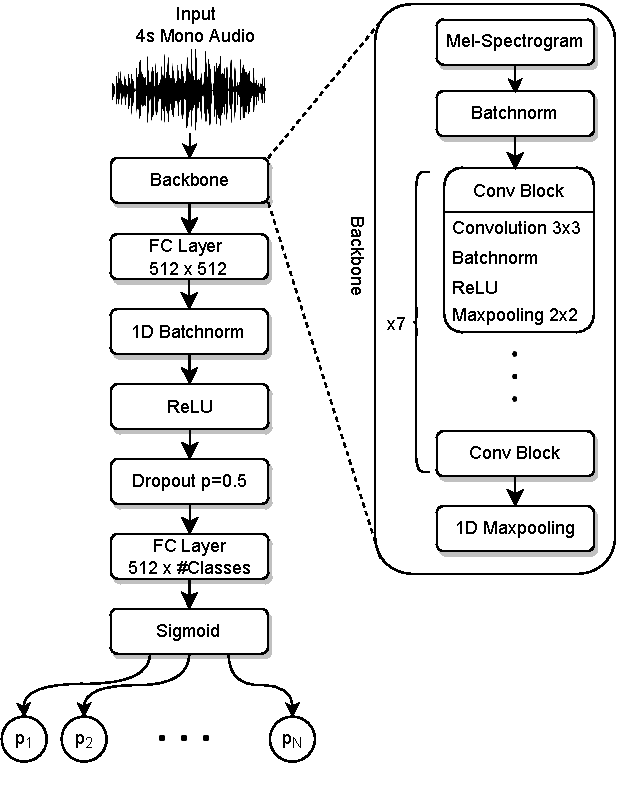
\includegraphics[width=6.5cm,height=8.0cm]{cnn_architecture_paperversion.pdf}}
	\end{minipage}
	\centering
	\vspace*{-0.6cm}
	\caption{Architecture of the CNN used for multi-instrument recognition.}
	\label{fig:architecture}
	\vspace*{-0.05cm}	
\end{figure}


\subsection{Data Resources}
\label{sec:method:data}
For TL, a combination of three multi-track datasets is used -- \textit{MedleyDB}~\cite{bittner2014medleydb} (including \textit{MedleyDB 2.0}~\cite{bittner2016medleydb2}), \textit{Mixing Secrets}~\cite{gururani2017mixingsecrets} and \textit{Slakh}~\cite{manilow2019slakh}. After discarding songs which exhibit severe crosstalk between the individual instrument tracks, the first two datasets both feature approximately 130 songs and the last one contains 2100 songs. Note that, although the \textit{Slakh} dataset is superior when it comes to size, several instruments sound quite unrealistic because all audio was synthesized from MIDI files using virtual instruments.  In addition to the three multi-track datasets, \textit{MTG-Jamendo}~\cite{bogdanov2019jamendo}, a large music tagging dataset is utilized for pre-training of all models. This music tagging dataset already comes with a predefined split. However, each multi-track dataset was randomly divided into training, validation and test set containing \SI{65}{\percent}, \SI{17.5}{\percent} and \SI{17.5}{\percent} of all songs, respectively. We made the decision to split the multi-track datasets at random for the sake of simplicity. This practice can potentially lead to overoptimistic results if songs from the same artist or album are contained in multiple splits. In order to reduce computation time, all audio data was converted to mono and downsampled to \SI{32}{\kilo\hertz}.

Since the three multi-track datasets used in this work exhibit different class structures, a unified instrument taxonomy has to be developed. Moreover, we want this taxonomy to be hierarchical in order to leverage relationships between instruments for learning broader concepts of musical instruments~\cite{garcia2021leveraging}. As a general rule for training DNNs, a sufficient number of examples for every class is required. In other words, classes with insufficient number of examples have to be discarded, which basically means that some information gets lost. However, our multi-track datasets are highly imbalanced and for certain instruments only few examples are available. To still utilize these underrepresented classes for training, our two-level hierarchy was defined as shown in Fig.~\ref{fig:taxonomy}. It is inspired by the \textit{Hornbostel-Sachs}~\cite{hornbostel1914systematik} system, which classifies musical instruments based on their underlying sound production mechanisms. As the physical principle of an instrument strongly correlates with its sound, such a taxonomy seems appropriate for our use case. The first level of our proposed taxonomy represents eight instrument families: voice, percussion, bowed string, plucked string, woodwind, brass, key and synth. The second level embodies seven specific instruments for which abundant data was available: singer, drums, violin, electric guitar, acoustic guitar, electric bass and piano. In total we have 15 classes.
\begin{figure}[t]
	\begin{minipage}[b]{1.0\linewidth}
		\centering
		\centerline{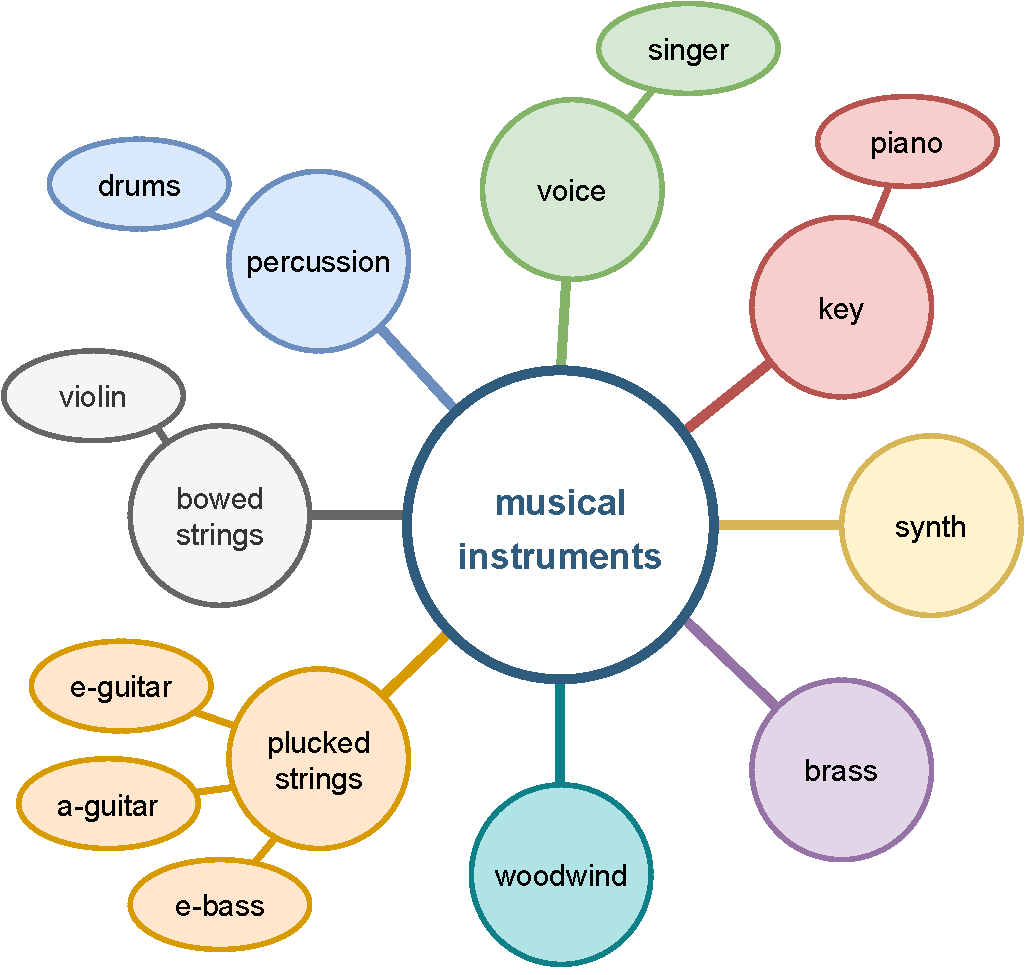
\includegraphics[width=7.0cm,height=6.25cm]{instrument-taxonomy-only15classes.pdf}}
	\end{minipage}
	\centering
	\caption{Two-level instrument taxonomy.}
	\label{fig:taxonomy}
	\vspace*{-0.05cm}	
\end{figure}

\subsection{Musical and Non-Musical Mixing}
\label{sec:method:dataloading}
Our main data augmentation approach is to create new unique mixtures out of the single-instrument tracks (sources) from the multi-track datasets. Therefore, we propose two mixing strategies -- \textit{musical mixing} and \textit{non-musical mixing}. Musical mixing means that only sources from the same song are combined to generate a new mixture, whereas non-musical mixing signifies that each source in a mix originates from a different song. The latter, which was successfully used in music source separation~\cite{uhlich2017improving}, obviously results in \enquote{non-musical}, strange sounding mixes, as each instrument plays in a different key and tempo. Nevertheless, the number of training examples can be increased massively by this mixing strategy, which in turn improves generalization. Musical mixing, on the other hand, naturally produces well-sounding results, since all sources originate from the same song and are therefore uniform in tempo and key. In order to investigate the performance of the two proposed mixing strategies, an experiment is conducted in Section~\ref{sec:experiments:mixing}. Note that for validation and testing, musical mixing was used exclusively, because in real-world recordings, instruments will almost always play in the same key and tempo. In the following paragraph, the data mixing approach is explained in more detail, illustrating how a polyphonic mixture is constructed from individual sources.

Initially, one of the three multi-track datasets is selected -- each one with the same probability of $1/3$. This step is necessary, because the \textit{Slakh} dataset is much larger than the other two multi-track datasets. Simply merging them and sampling from the combined dataset would lead to a domination of \textit{Slakh} samples. However, this should be avoided, because, as already mentioned, the \textit{Slakh} dataset is synthesized from MIDI files and is therefore not the best to represent real-world music recordings. In the next step, one of the two proposed mixing strategies is selected. Musical mixing is applied with probability $p_{musical}$ and non-musical mixing is used with probability $1 - p_{musical}$. Then we choose the number of sources $N$ in the mixture. As our models should be able to cope with solo-instrument recordings as well, we load single sources ($N=1$) with a certain probability $p_{single-source}$. After that, the following steps are performed $N$ times for the non-musical mixing method: select a song, select a source from this song, select a four-second chunk from this source, apply some digital audio effects on the audio and add it to the mixture. Four digital audio effects from the \textit{audiomentations}~\cite{audiomentations} library are utilized -- each one with a certain probability: amplitude scaling (gain), three types of filters (high shelf, low shelf and peaking filter), pitch shifting and time stretching. The order of these effects as well as all their parameters are random. Note that, in the musical mixing case, all sources originate from the same song, hence a song is selected only once and not $N$ times (at every loop iteration). Furthermore, the time position of all chunks has to be identical in order to obtain musical sounding results. Finally, pitch shifting and time stretching are omitted for the same reason when musical mixing is applied.

\subsection{Transfer Learning (TL)}
\label{sec:method:training}
TL is the procedure of applying knowledge gained from solving one task to another, related task~\cite{tan2018survey}. CNNs typically learn general concepts -- like detecting edges or simple shapes -- in the earlier layers and increasingly more complex, task-specific concepts in the later layers. Therefore, the first convolutional layers can easily be reused for a similar task. If source and target tasks are related, such as music tagging and multi-instrument recognition, even a complete transfer of all convolutional layers can be considered~\cite{ribani2019survey} as for both tasks, the CNN has to identify similar patterns in mel-spectrograms.

In order to train our classifier, we experimented with two TL methods. For both approaches, we first replaced the fully connected layers of the pre-trained model with new, randomly initialized ones. Furthermore, the size of the output layer was adjusted to 15 to suit the target task of predicting eight instrument families and seven explicit instruments, according to the taxonomy proposed in Section~\ref{sec:method:data}. During training with the multi-track data, we either (1) froze the whole backbone network and only retrained the fully connected layers or (2) allowed the backbone to be learnable as well, but with a smaller learning rate than the fully connected layers. As a third method (3) the entire model is trained with the multi-track data from scratch, i.e. not utilizing the pre-trained weights obtained by training with~\textit{MTG-Jamendo}. Strictly speaking, method (3) has nothing to do with TL, nevertheless we use it as a reference to show the benefits of methods (1) and (2). The results of these three experiments are discussed in Section~\ref{sec:experiments:tl}.


\section{Experiments}
\label{sec:experiments}

\subsection{Experimental Setup}
\label{sec:experiments:setup}
Prior to all experiments, a CNN is trained on the 50 most popular tags from the~\textit{MTG-Jamendo} dataset. The following experiments use this pre-trained model as a starting point for TL. Since we generate training examples on-the-fly when working with the multi-track data, the concept of epochs -- a complete pass over the training set -- does not exist. Therefore, we defined the transit of 1920 samples (120 batches of size 16) as one epoch. After each epoch, the model is evaluated on the validation set and at the end of training (after 150 epochs), the model with the lowest validation loss is retained. For all experiments, the ADAM optimizer in combination with a step-wise learning rate scheduler was employed. Every 20 epochs the learning rate was reduced by a constant factor of $0.3$. Binary cross-entropy served as a loss function. For testing, 120 \textit{musical} mixtures were created on-the-fly from the individual instrument tracks contained in the test splits of the three multi-track datasets. %Mixes for testing are generated using the musical mixing strategy, as this strategy results in mixes, which are very close to real-world recordings. To ensure reproducibility and enable the comparison of different models, seeds of the random number generators are fixed.

\subsection{Transfer Learning (TL) Results}
\label{sec:experiments:tl}
We investigate the three TL methods proposed in Section~\ref{sec:method:training}. Each model was evaluated on the testing data and area under the receiver operating characteristic curve (ROC-AUC), area under the precision-recall curve (PR-AUC)~\cite{davis2006relationship} and test loss were computed. For all three TL methods, $0.01$ was chosen as an initial learning rate for the fully connected layers. When training from scratch, the same learning rate was used for the backbone as well. For the fine-tuning approach, the learning rate of the backbone was initialized with $0.0001$. The ratio between muscial and non-musical mixes $p_{musical}$ was set to $0.6$ for this experiment.

Table~\ref{tab:transfer-learning-experiment} contains the results of the three TL experiments. Unsurprisingly, the performance is worst when no pre-training is exploited and the model is trained from scratch (i.e. \emph{From Scratch}) on the multi-track data. Utilizing a pre-trained backbone with frozen parameters (i.e. \emph{Frozen Backbone}) significantly increases the performance, indicating that pre-training on a large-scale dataset is beneficial indeed. However, fine-tuning the weights of the backbone (i.e. \emph{Fine-tuned}) to fit the needs of the target task yields additional performance gains.

\begin{table}[h]
	\centering
	\resizebox{0.4\textwidth}{!}{
	\centering
	\begin{tabular}{c|c|c|c}
		& ROC-AUC & PR-AUC & Test Loss\\ \hline
		From Scratch  & 0.8488 & 0.6812 & 0.4459\\ \hline
		Frozen Backbone  & 0.8908  & 0.7623 & 0.4160\\ \hline
		Fine-tuned & 0.9429  & 0.8334 & 0.3618\\
	\end{tabular}}
	\caption{ROC-AUC, PR-AUC and test loss for different TL approaches.}
	\label{tab:transfer-learning-experiment}
\end{table}

\subsection{Mixing Strategy}
\label{sec:experiments:mixing}
Our data augmentation technique (see Section~\ref{sec:method:dataloading}), is based on mixing of individual sources to create new examples for training. For this reason, the two mixing strategies musical mixing with probability $p_{musical}$ and non-musical mixing with probability $1 - p_{musical}$ are used. To determine the best ratio between these two methods, we experimented with different values for the hyperparameter $p_{musical}$. As depicted in Fig.~\ref{fig:mixing-strategy}, the best performance was obtained for $p_{musical}=0.4$. The result of this investigation suggests, that neither mixing strategy is superior, but rather a combination of both works best. Using only the non-musical mixing approach results in a larger variation of the training examples. However, the model does not get the chance to learn how to identify sources in \enquote{real} music where all instruments play in the same key and tempo. In this case, instrument recognition is usually more difficult though, at least for us humans, since masking of individual sources is more pronounced due to synchronous note onsets and overlapping partials. Although overlapping of partials results in consonant sounds, it is substantially harder to distinguish individual sources in this case. On the other hand, if only the musical mixing approach is utilized, fewer variation in the training examples can be created, as the number of possible combinations of sources from a single song is limited. This in turn can lead to poorer generalization of the model. We infer from this experiment, that a blend of both mixing strategies is optimal for multi-instrument recognition.
\begin{figure}[t]
	\begin{minipage}[b]{0.8\linewidth}
		\centering
		\centerline{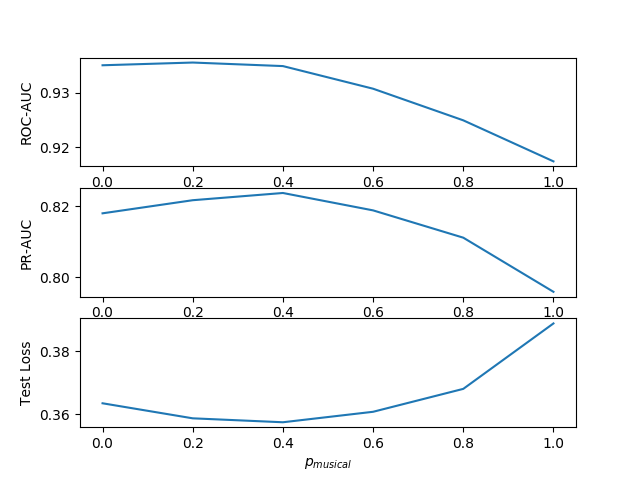
\includegraphics[width=9.25cm,height=8.0cm]{p_mult_songs-experiment.png}}
	\end{minipage}
	\centering
	\vspace*{-0.6cm}
	\caption{ROC-AUC, PR-AUC and test loss for different values of $p_{musical}$.}
	\label{fig:mixing-strategy}
	\vspace*{-0.05cm}	
\end{figure}

\subsection{Performance of the Classifier}
\label{sec:experiments:performance}
After setting the classification threshold for the sigmoid activations of the CNN outputs to $0.35$ -- this value maximizes the F1-score -- we are able to report threshold-dependent metrics. Fig.~\ref{fig:classifier-performance} shows the class-wise F1-scores and accuracies of our final model. Unsurprisingly, classes with abundant training data, such as percussion, drums or plucked strings, exhibit the best F1-scores, while identification of instruments or families with insufficient data, like brass, woodwind or violin, does not work well. Note that the F1-score for the brass class is zero because the number of true positives is zero. In addition to F1-scores, we also report the class-wise accuracy. However, accuracy has to be used with caution, since it is highly dependent on the distribution of the dataset. For example, a high accuracy for the brass class is obtained, completely hiding the fact that not a single brass instrument was identified correctly. Instead, the model always predicts the absence of the brass family, which is true most of the time, since the brass class is very poorly represented in the data. Apart from that, we obtained state-of-the-art performance for the majority of classes. With F1-scores above \SI{95}{\percent} for some classes, our classifier can easily compete with other recent multi-instrument recognition systems from the literature~\cite{gururani2019attention, seipel2018music, kadandale2018musical}. Unfortunately, performances reported by different researchers are generally hard to compare since there is no benchmark dataset for multi-instrument recognition.

\begin{figure}[htb]
\begin{center}
	\begin{minipage}[b]{0.8\linewidth}
		\centering
		\centerline{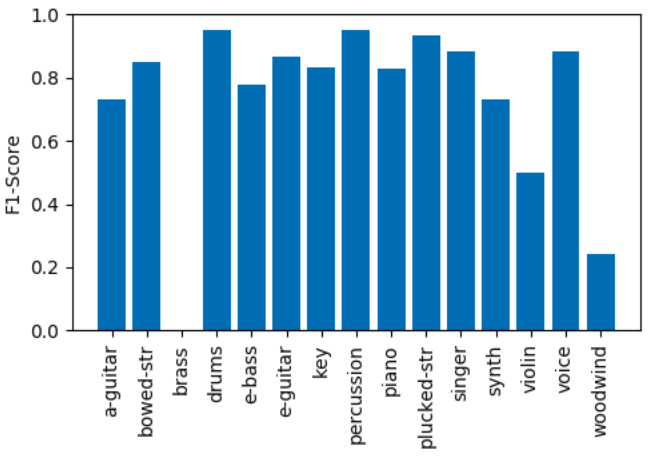
\includegraphics[width=7.5cm]{f1-scores.png}}
		  \vspace{0.1cm}
		%\centerline{(a) F1-score}\medskip
	\end{minipage}
	\begin{minipage}[b]{0.8\linewidth}
		\centering
		\centerline{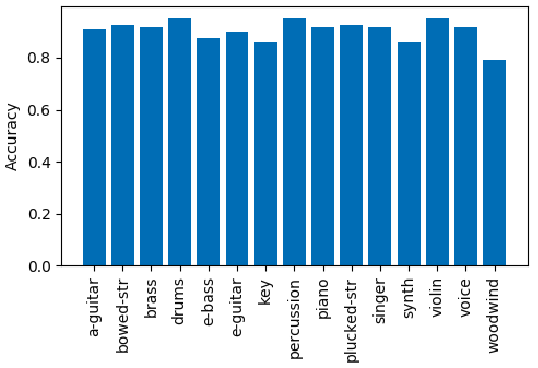
\includegraphics[width=7.5cm]{accuracy.png}}
		%  \vspace{1.5cm}
		%\centerline{(b) accuracy}\medskip
	\end{minipage}
	\caption{Class-wise F1-score and accuracy of the classifier.}
	\label{fig:classifier-performance}
 \end{center}
\end{figure}
\vspace{-3mm}
\section{Conclusion}
\label{sec:conclusion}
In this paper, we investigated how different TL methods perform when transferring pre-trained CNNs to the task of multi-instrument recognition. We show that pre-training on a music tagging dataset yields significant performance gains. For TL, training the fully connected layers from scratch and fine-tuning the convolutional layers worked best. Furthermore, we explored musical and non-musical mixing as strategies to generate training examples. For the task of multi-instrument recognition, a combination of both mixing strategies -- using \SI{40}{\percent} musical mixtures and \SI{60}{\percent} non-musical mixtures -- turned out to be ideal. In the end, we evaluated our final model and obtained class-wise F1-scores above \SI{95}{\percent} for some classes, which is state-of-the-art for instrument recognition in polyphonic recordings.






% References should be produced using the bibtex program from suitable
% BiBTeX files (here: strings, refs, manuals). The IEEEbib.bst bibliography
% style file from IEEE produces unsorted bibliography list.
% -------------------------------------------------------------------------
\bibliographystyle{IEEEbib}
\bibliography{refs}
%\printbibliography

\end{document}
